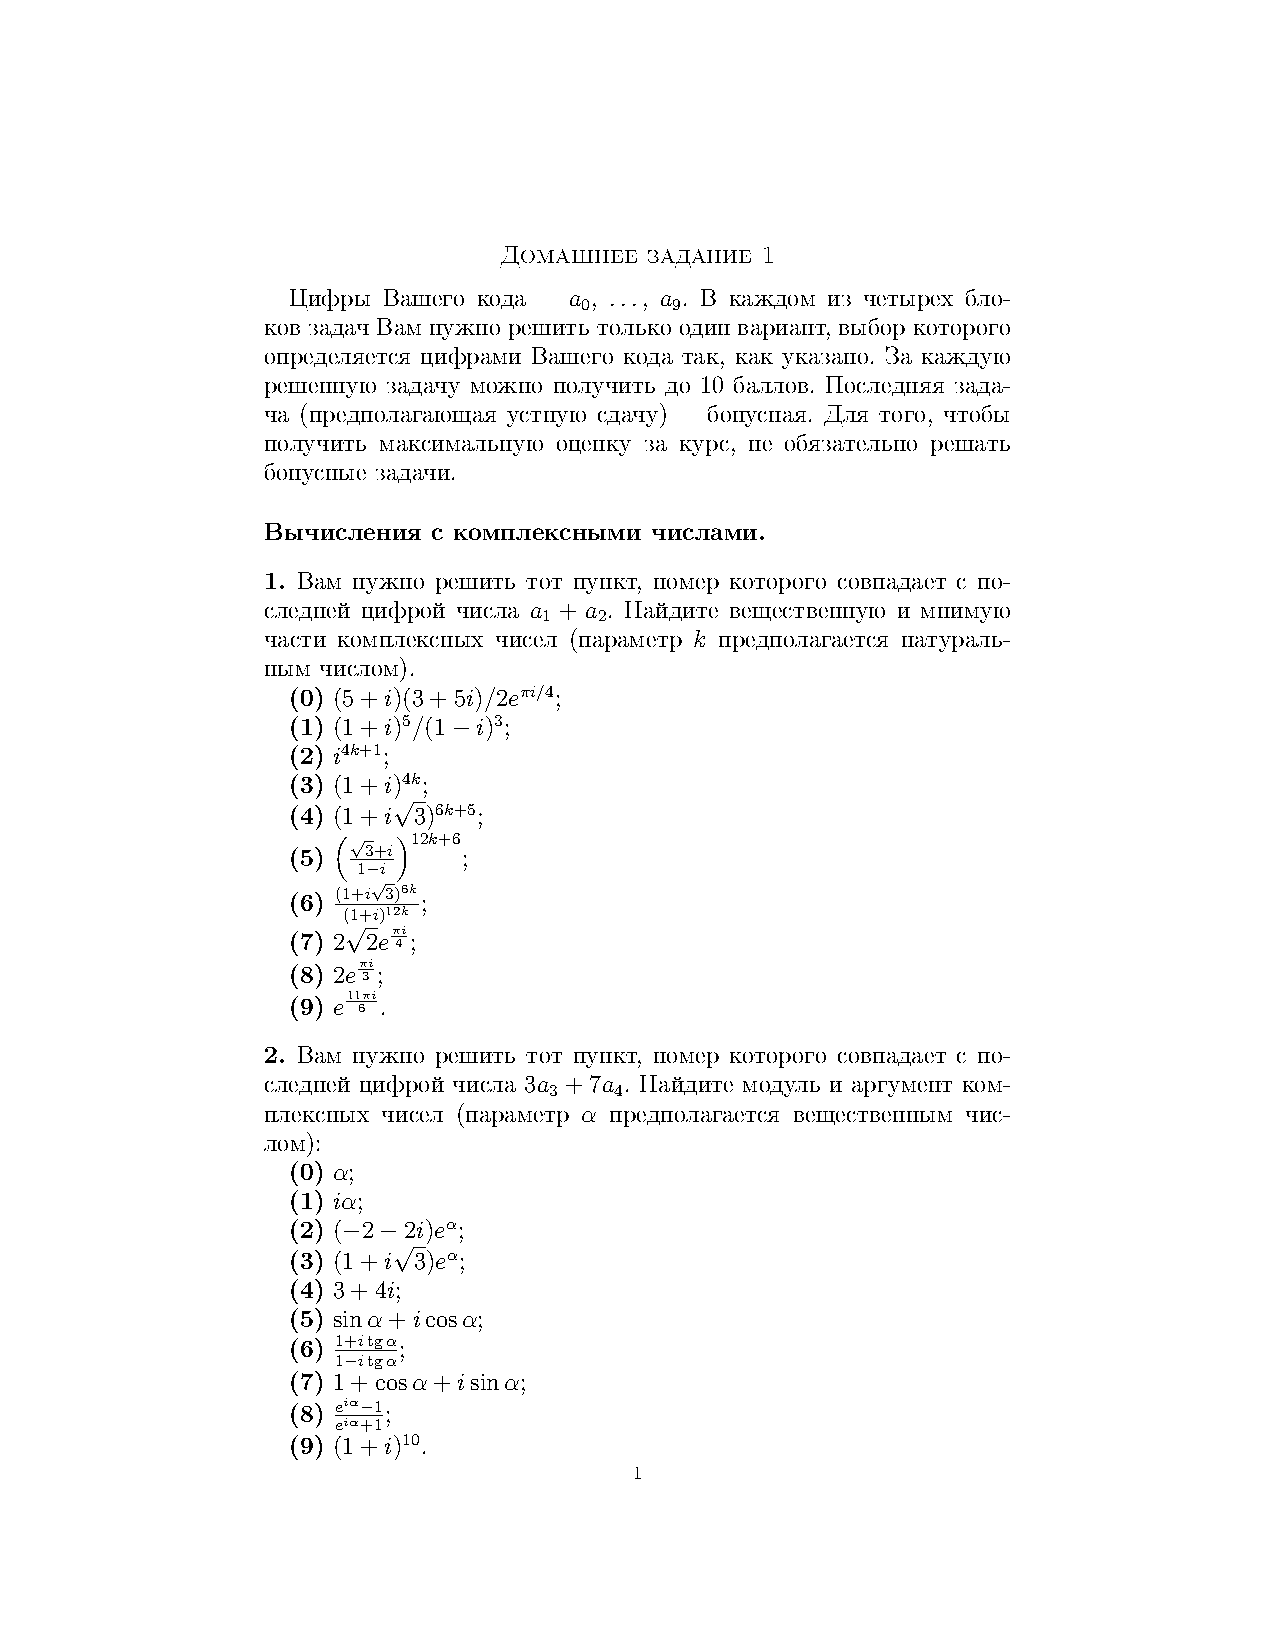
\includepdf[scale=1,pages=1-3]{Tasks/hw1}
\newpage
\section*{Решения}
\subsection*{Задача 1}
	необходимо решить пункт под номером $7 + 8 = 5 \mod 10$
	\begin{gather*}
		\left(\frac{\sqrt{3} + i}{1 - i}\right)^{12k + 6}\\
		\left(\frac{\sqrt{3} + i}{1 - i}\right)^2 = 
		\frac{2 + 2\sqrt{3} i}{-2i} = -\frac{1 + \sqrt{3}i}{i} = 
		i - \sqrt{3}\\
		\left(1^2 + \sqrt{3}^2\right)^{\frac{1}{2}} = 
		2\qquad \sin(\theta) = 
		\frac{1}{2},\ \cos(\theta) = 
		\frac{-\sqrt{3}}{2}\ \Rightarrow\ \theta = 
		\frac{5\pi}{6}\\
		\left(\frac{\sqrt{3} + i}{1 - i}\right)^{12k + 6} = 
		\left(\frac{\sqrt{3} + i}{1 - i}\right)^{12k} \cdot \left(\frac{\sqrt{3} + i}{1 - i}\right)^{6} = 
		(-64)^k \cdot 8i = (-1)^k 2^{6k+3} i
	\end{gather*}
\vskip 0.4in

\subsection*{Задача 2}
	необходимо решить пункт под номером $3 \cdot 9 + 7 \cdot 7 = 6 \mod 10$
	\begin{gather*}
		\frac{1 + i \tan \alpha}{1 - i \tan \alpha} = 
		\frac{1 + i \frac{e^{i \alpha} - e^{-i \alpha}}{i(e^{i \alpha} + e^{-i \alpha})}}{1 - i \frac{e^{i \alpha} - e^{-i \alpha}}{i(e^{i \alpha} + e^{-i \alpha})}} =
		\frac{1 + \frac{e^{i \alpha} - e^{-i \alpha}}{e^{i \alpha} + e^{-i \alpha}}}{1 - \frac{e^{i \alpha} - e^{-i \alpha}}{e^{i \alpha} + e^{-i \alpha}}} =
		\frac{\frac{(e^{i \alpha} + e^{-i \alpha}) + (e^{i \alpha} - e^{-i \alpha})}{e^{i \alpha} + e^{-i \alpha}}}{\frac{(e^{i \alpha} + e^{-i \alpha}) - (e^{i \alpha} - e^{-i \alpha})}{e^{i \alpha} + e^{-i \alpha}}} =
		\frac{(e^{i \alpha} + e^{-i \alpha}) + (e^{i \alpha} - e^{-i \alpha})}{(e^{i \alpha} + e^{-i \alpha}) - (e^{i \alpha} - e^{-i \alpha})} =\\
		\frac{2e^{i \alpha}}{2e^{-i \alpha}} = e^{2i\alpha} = \cos(2x) + i\sin(2x)\\
		\operatorname{mod} (e^{2i\alpha}) = 1\qquad
		\operatorname{arg} (e^{2i\alpha}) = 2\alpha
	\end{gather*}
\vskip 0.4in

\subsection*{Задача 3}
	необходимо решить пункт под номером $2 \cdot 9 + 3 = 1 \mod 10$
	\begin{gather*}
		\cos(5x) + i \sin(5x) = 
		(\cos(x) + i \sin(x))^5 =\\
		\cos(x)^5 - 10 \sin(x)^2 \cos(x)^3 + 5\sin(x)^4 \cos(x) + i(\sin(x)^5 - 10\sin(x)^3 \cos(x)^2 + 5 \sin(x)\cos(x)^4) =\\
		\\
		\cos(x)^5 - 10(1 - \cos(x)^2)\cos(x)^3 + 5(1-\cos(x)^2)^2\cos(x) +\\ i(\sin(x)^5 - 10 \sin(x)^3(1-\sin(x)^2) + 5 \sin(x)(1-\sin(x)^2)^2) =\\
		\\
		16\cos(x)^5 - 20 \cos(x)^3 + 5\cos(x) + i(16\sin(x)^5 - 20\sin(x)^3 + 5\sin(x))\\
		\cos(5x) = 16 \cos(x)^5 - 20 \cos(x)^3 + 5\cos(x)
	\end{gather*}
\vskip 0.4in

\subsection*{Задача 4}
	необходимо решить пункт под номером $8 + 6 = 4 \mod 10$
	\begin{gather*}
		z^3 = i\\
		z^3 - i = 0\\
		z^3 + i^3 = 0\\
		(z + i)(z^2 - iz - 1) = 0\\
		z_1 = -i,\ z_2 = \frac{1}{2}(i - \sqrt{3}),\ z_3 = \frac{1}{2}(i + \sqrt{3})
	\end{gather*}
\vskip 0.4in


\subsection*{Задача 5}
	необходимо решить пункт под номером $7 + 6 = 3 \mod 10$\\
	Заметим что многочлен $f(x)$ можно представить в виде $f(x) = A q_1(x)\ldots q_k(x) (x-x_1)^{n_1} \ldots (x - x_r)^{n_r} (x - y_1)^{m_1} \ldots (x - y_s)^{m_s}$, где $q_i$ -- квадратные многочлены без вещественных корней, $n_i$ -- четные степени (пусть $n_i = 2d_i$), $m_i$ -- нечетные степени, а также $A \ne 0$. Заметим что так как $f(x) \geqslant 0$, то $m_i = 0$, а следовательно $f(x) = A q_1(x)\ldots q_k(x) (x-x_1)^{n_1} \ldots (x - x_r)^{n_r}$, если в таком разложении какие-то $q_i$ отрицательны при всех $x$, вынесем $-1$ из них в $A$, тогда получим $f(x) = \tilde{A} \tilde{q_1}(x)\ldots \tilde{q_k}(x) (x-x_1)^{n_1} \ldots (x - x_r)^{n_r}$. Так как $\tilde{q_i} > 0$, то $(x - x_i)^{n_r} \geqslant 0$ для всех $x$, тогда также $\tilde{A} > 0$. Тогда можно представить $\tilde{q_i}$ как сумму 2 кадваратов*, а также заметить, что $(x - x_i)^{n_i} = ((x - x_i)^{d_i})^{2}$.\\
	Осталось заметить, что если $A(x) = a_1(x)^2 + a_2(x)^2$ и $B(x) = b_1(x)^2 + b_2(x)^2$, то
	\begin{gather*}
		A(x)B(x) = a_1(x)^2b_1(x)^2 + a_1(x)^2b_2(x)^2 + a_2(x)^2b_1(x)^2 + a_2(x)^2b_2(x)^2\\
		= (a_1(x)^2b_1(x)^2 + 2a_1(x)a_2(x)b_1(x)b_2(x) + a_2(x)^2b_2(x)^2) + (a_1(x)^2b_1(x)^2 - 2a_1(x)a_2(x)b_1(x)b_2(x) + a_2(x)^2b_2(x)^2)\\
		= (a_1(x)b_1(x) + a_2(x)b_2(x))^2 + (a_1(x)b_1(x) - a_2(x)b_2(x))^2
	\end{gather*}
	То есть произведение сумм квадратов можно представить в виде суммы квадратов, а следовательно, представив $f(x)$ в виде суммы квадратов, мы разбили $f(x)$ на сумму квадратов.\\
	Осталось представить $\tilde{q_i}$ в виде суммы квадратов -- пусть $\tilde{q_i} = a\left(x^2 + \frac{b}{a}x + \frac{c}{a} \right)$, тогда
	\begin{gather*}
		a\left(x^2 + \frac{b}{a}x + \frac{c}{a}\right)\\
		= a \left(x^2 + \frac{bx}{a} + \left(\frac{b}{2a}\right)^2 - \left(\frac{b}{2a}\right)^2 + \frac{c}{a}\right)\\
		= a\left(\left(x + \frac{b}{2a}\right)^2 - \left(\frac{b}{2a}\right)^2 + \frac{c}{a}\right)\\
		= a\left(x + \frac{b}{2a}\right)^2 + a\left(-\left(\frac{b}{2a}\right)^2 + \frac{c}{a}\right)\\
		= \left(\sqrt{a}\left(x + \frac{b}{2a}\right)\right)^2 + \left(-a\left(\frac{b}{2a}\right)^2 + c\right)\\
		= \left(\sqrt{a}\left(x + \frac{b}{2a}\right)\right)^2 + \frac{4ac - b^2}{4a}
	\end{gather*}
	Таким образом мы представили все элементы разложения в виде сумм квадратов, а, следовательно, показали что любой неотрицательный вещественный многочлен от одной переменной можно представить в виде суммы двух квадратов